\documentclass[a4paper,14pt]{article}
\usepackage[a4paper, mag=1000, left=2.5cm, right=1cm, top=2cm, bottom=2cm, headsep=0.7cm, footskip=1cm]{geometry}
\usepackage[utf8]{inputenc}
\usepackage[T2A]{fontenc}
\usepackage[english,russian]{babel}
\usepackage{indentfirst}
%\usepackage[dvipsnames]{xcolor}
\usepackage[colorlinks]{hyperref}
\usepackage{amsfonts} 
\usepackage{amsmath}
\usepackage{graphicx}
\usepackage{float}

\DeclareGraphicsExtensions{.png,.jpg}

\usepackage{fancyhdr}
\pagestyle{fancy}
\fancyhead[LE,RO]{\thepage}
\fancyfoot{}

\usepackage{listings}

\hypersetup{linkcolor=black}

\title{non-linear equations}
\author{Иван Золин}
\date{2023}
\thispagestyle{empty}
\begin{document}
	
	\begin{titlepage}
		\begin{center}
			\textsc{
				Санкт-Петербургский политехнический университет имени Петра Великого \\[5mm]
				Физико-механический институт\\[2mm]
				Высшая школа прикладной математики и физики            
			}   
			\vfill
			\textbf{\large
				Интервальный анализ\\
				Отчёт по лабораторной работе №3 \\[3mm]
			}                
		\end{center}
		
		\vfill
		\hfill
		\begin{minipage}{0.5\textwidth}
			Выполнил: \\[2mm]   
			Студент: Золин Иван \\
			Группа: 5030102/00201\\
		\end{minipage}
		
		\hfill
		\begin{minipage}{0.5\textwidth}
			Принял: \\[2mm]
			к. ф.-м. н., доцент \\   
			Баженов Александр Николаевич
		\end{minipage}
		
		\vfill
		\begin{center}
			Санкт-Петербург \\2023 г.
		\end{center}
	\end{titlepage}
	
	\tableofcontents
	\newpage
	
	\section{Постановка задачи}
	Задана система нелинейных уравнений:
	\begin{equation*}
		\begin{cases}
			x^2 + y^2 = 1\\
			x = y^2
		\end{cases}
	\end{equation*}
	Необходимо найти корни данной системы точеченых нелинейных уравнений, используя интервальный метод Кравчика.
	
	\section{Теория}
	\subsection{Внешнее множество решений}
	Внешним множеством решений называется объединенное множество решений, образованное решениями всех точечных систем $F(a,x)=b$
	\begin{equation} \label{UniSet}
		\Xi_{\mathrm{uni}}(\textbf{F},\textbf{a}, \textbf{b})=\{x\in\mathbb{R}^n\;|\;(\exists a\in\textbf{a})(\exists b\in\textbf{b})(F(a,x)=b)\}
	\end{equation}
	
	\subsection{Метод Кравчика}
	Метод Кравчика предназначен для уточнения двухсторонних границ решений систем уравнений, в общем случае нелинейных, заданных на некотором брусе $\textbf{X}\subset \mathbb{IR}$, вида
	\begin{equation}
		F(x)=0, \quad \textup{где} \;\; F(x)=\{F_1(x),...,F_n(x)\}^T,\; x=(x_1,...x_n)
	\end{equation}
	Также данный метод может быть использован для того, чтобы понять, что решений нет.\\
	Отображение $\mathcal{K}:\mathbb{ID}\times\mathbb{R}\rightarrow\mathbb{IR}^n$, задаваемое выражением
	\begin{equation}
		\mathcal{K}(\textbf{X}, \overline{x}):=\overline{x}-\Lambda*F(\overline{x})-(I-\Lambda*\textbf{L}*(\textbf{X}-\overline{x})
	\end{equation}
	называеся оператором Кравчика на $\mathbb{ID}$ относительно точки $\overline{x}$.\\
	Итерационная схема данного метода выглядит следующим образом
	\begin{equation}
		\textbf{X}^{k+1}\leftarrow\textbf{X}^k\cap\mathcal{K}(\textbf{X}^k, \overline{x}^k), \;\; k=0,1,2..., \; x^k\in\textbf{X}^k
	\end{equation}
	Сходимость данного метода гарантирована при выполнении условия
	\begin{equation}
		\rho(I-\Lambda*\textbf{L})<1 - \textup{спектральный радиус меньше единицы}
	\end{equation}
	Частным случаем данного метода является линейный метод Кравчика, итерационная схема которого выглядит следующим образом:
	\begin{equation}
		\textbf{x}^{k+1}=\left(\Lambda*\textbf{b}+(I-\Lambda*\textbf{A})*\textbf{x}^k\right)\cap\textbf{x}^{k}
	\end{equation}
	$\textbf{A}$ в данном случае является интервальной матрицей коэффициентов соответсвующей ИСЛАУ, а $\textbf{b}$ - вектором свободных членов.\\
	В случае линейности системы и выполнения условия $\eta=||I-\Lambda*\textbf{A}||_\infty\leq 1$ в качестве начального приближения можно взять брус 
	\begin{equation}
		\textbf{x}^0=([-\theta,\theta],...,[-\theta,\theta])^T, \quad \textup{где}  \;\theta=\frac{||\Lambda \textbf{b}||_\infty}{1-\eta}
	\end{equation}
	
	\section{Результаты}
	\begin{figure}[H] \label{MatrixCorrSet}
		\centering
		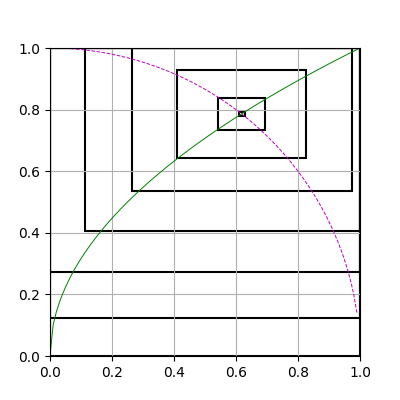
\includegraphics[width=0.5\textwidth]{g.png}
		\caption{Метод Кравчика - пересечение параболы и окружности} 
	\end{figure}
	
	Получим таблицу результатов для некотрых $\mathbf{X}_1, \mathbf{X}_2$
	\begin{table}[H]
		\begin{center}
			\begin{tabular}{|c|c|c|c|c|}
				\hline
				№ & $\mathbf{X}_2$ & $\mathbf{X}_1$ & ширина $\mathbf{X}_1$ &  ширина $\mathbf{X}_2$ \\
				\hline
				1   &[0, 1]  & [0, 1] & 1.0 & 1.0 \\
				2   &$[0, 1]$  & $[0.125, 1]$ & 0.875 & 1.0 \\
				3   &$[0.111684, 1] $ & $[0.406219, 1]$ & 0.0.5937 & 0.8883\\
				4   &$[0.266059, 0.973673]$ & $[0.534126, 1]$ & 0.4658 & 0.7076\\
				5   &$[0.409351, 0.82672]$ & $[0.64279, 0.92999] $ & 0.2871 & 0.4173\\
				6   &$[0.542195, 0.693873] $& $[0.735163, 0.83714]$& 0.1020 & 0.1517 \\
				7   &$[0.608239, 0.627829]$ & $[0.779572, 0.79273]$ & 0.0132 & 0.0196\\
				8   &$[0.617871, 0.618197]$ & $[0.786042, 0.786261]$ & 0.000219 & 0.0003264\\
				9   &$[0.618034, 0.618034]$ &$ [0.786151, 0.786151]$ & $6.08*10^{-8}$ &  $9.06*10^{-8}$\\
				\hline
			\end{tabular}
		\end{center}
	\end{table} 
	
	\section{Вывод}
	\begin{enumerate}
		\item Полученные результаты подтверждают эффективность и сходимость интервального метода Кравчика для решения системы нелинейных уравнений. На каждой итерации метода границы решений сужаются, итерации продолжаются до достижения требуемой точности.
		\item Точное решение системы $x = 0.6180339, y = 0.7861513$ совпадает с результатами, полученными методом. Таким образом, метод успешно находит корни системы нелинейных уравнений.
		\item На 9 итерации метод дошел до  $2.52*e^{-18}\; $ и $\; 2.46*e^{-17}$ соответсвенно
		\item Заметим, что сходимость метода обеспечивается выполнением условия $\rho(I-\Lambda*\textbf{L})<1$, что подчеркивает важность выбора подходящих параметров и начальных условий для успешной работы метода.
	\end{enumerate}
	
	\newpage
	\addcontentsline{toc}{section}{Литература}
	
	\begin{thebibliography}{4}
		\bibitem{s:hist}
		Histogram. URL: \url{https://en.wikipedia.org/wiki/Histogram}
		\bibitem{b:probSectMath}
		Вероятностные разделы математики. Учебник для бакалавров технических направлений.//Под ред. Максимова Ю.Д. --- Спб.: «Иван Федоров», 2001. --- 592 c., илл.
		\bibitem{s:boxplot}
		Box plot. URL: \url{https://en.wikipedia.org/wiki/Box_plot}
		\bibitem{a:nonParamRegr}
		Анатольев, Станислав (2009) «Непараметрическая регрессия», Квантиль, №7, стр. 37-52.
	\end{thebibliography}
	
\end{document}